\documentclass{standalone}

\usepackage{setspace}
\usepackage{times}
\usepackage{amsmath}
\usepackage{amssymb}
\usepackage{xparse}
\usepackage{ifthen}

\usepackage[dvipsnames]{xcolor}
\usepackage{tikz}
\usetikzlibrary{arrows,calc,patterns,patterns.meta}
\pgfdeclarelayer{background}
\pgfdeclarelayer{foreground}
\pgfsetlayers{background,main,foreground}

\usepackage{pgfplots}
\pgfplotsset{compat=1.15}

\definecolor{red}{HTML}{972e21}
\definecolor{yellow}{HTML}{ebb83f}
\definecolor{blue}{HTML}{5e7fbf}
\definecolor{green}{HTML}{5fd94e}
\renewcommand{\seriesdefault}{\bfdefault}
\renewcommand{\familydefault}{\sfdefault}

\begin{document}
    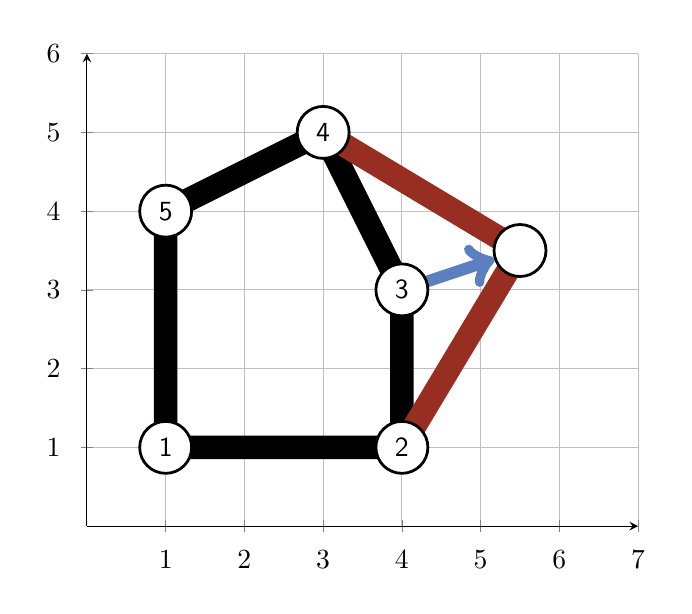
\begin{tikzpicture}[x=1cm,y=1cm,every node/.style={circle,inner sep=0pt,line width=1pt, minimum size = 0.66cm}]
        \begin{axis}[
            x=1.0cm,y=1.0cm,
            axis lines=middle,
            ymajorgrids=true,
            xmajorgrids=true,
            xmin=0,
            xmax=7,
            ymin=0,
            ymax=6,
            xtick={0.0,...,7.0},
            ytick={0.0,...,7.0},]  
            \begin{pgfonlayer}{foreground}
                \node[draw,fill=white] at (1cm,1cm) (v1) {1};
                \node[draw,fill=white] at (4cm,1cm) (v2) {2};
                \node[draw,fill=white] at (4cm,3cm) (v3) {3};
                \node[draw,fill=white] at (3cm,5cm) (v4) {4};
                \node[draw,fill=white] at (1cm,4cm) (v5) {5};
                \node[draw,fill=white] at (5.5cm,3.5cm) (v6) {};
            \end{pgfonlayer}
            \draw[-,line width=0.3cm,line join=round,black] (v1.center) -- (v2.center) -- (v3.center) -- (v4.center) -- (v5.center) -- (v1.center);
            \draw[-,line width=0.3cm,line join=round,red] (v2.center) -- (v6.center) -- (v4.center);
            \draw[->,line width=0.15cm,line join=round,blue] (v3.center) -- (v6);
        \end{axis}
    \end{tikzpicture}
\end{document} 
